\chapter{驾驶人行为特性的内涵}
最简单的跟驰行为可以划分为三个子行为,感知与信息收集,驾驶决策和对车辆的操控。
感知与信息收集过程中,驾驶人主要依靠视觉采集相关的信息,这些信息来源于引导车辆和自身车辆。驾驶人只对部分信息变量敏感,包括速度,加速度,跟驰距离,相对速度,以及这些变量的某些函数(如时间间隔)。
驾驶人收集到信息后通过采样与整合对这些信息进行解释,这种解释依靠驾驶人的对于车辆动态特性的理解以及其积累的驾驶经验。通过对信息解释的整合处理,最终形成驾驶决策。
驾驶决策形成后,驾驶人通过对车辆机件的操作,对车辆的动态施加控制。跟驰过程框图如


\begin{figure}[htpb]
	\centering
	\label{following_blockdia}
	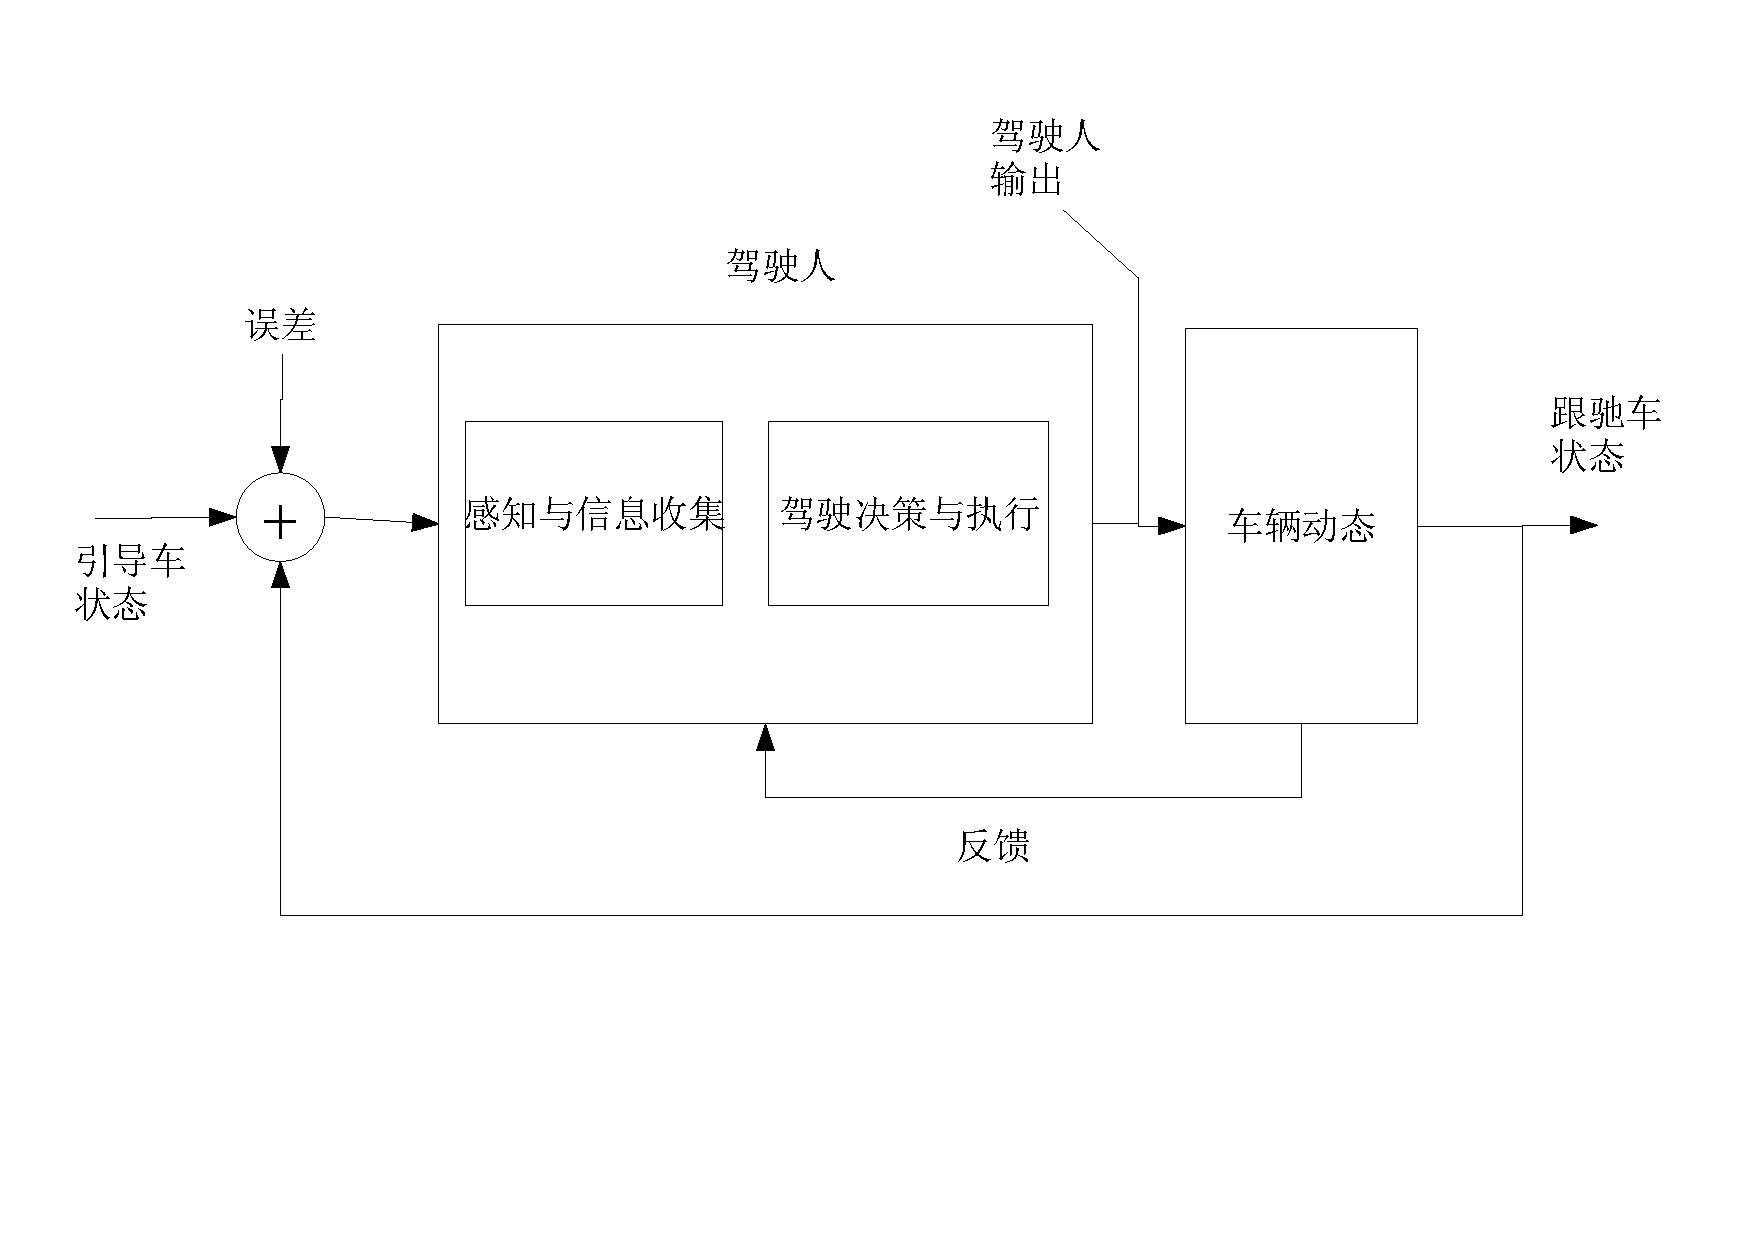
\includegraphics[totalheight=10cm]{following_blockdia}
	\caption{跟驰过程框图}
\end{figure}

驾驶人行为可以分为跟驰行为和变道行为,两者
%\begin{table}[htbp]
% \centering
% \caption{Add caption}
% \begin{tabular}{cccc}
%   \addlinespace
%    \toprule
%    Face database & Yale  & Caltech & ORL \\
%    \midrule
%    Number of training & \multicolumn{ 1}{c}{5} & \multicolumn{ 1}{c}{3} & \multicolumn{ 1}{c}{3} \\
%    samples per class  & \multicolumn{ 1}{c}{} & \multicolumn{ 1}{c}{} & \multicolumn{ 1}{c}{} \\
%    \bottomrule
%    \end{tabular}
%  \label{tab:addlabel}
%\end{table}

\section{跟驰行为特性}
(注意这里所指的)
\subsection{跟驰行为特性参数}
描述微观的驾驶人跟驰行为时,对于每一个人车单元DVU(driver-vehicle-unit)有若干的特性参数来反映驾驶人的行为,这些参数包括两类,一类是可以直接测量或经由计算所得的变量,直接测量的变量包括人车单元DVU的即时速度,即时加速度,相对速度和跟驰距离。由直接测量变量经过计算得出的变量,包括跟车对的时间间隔,视觉扩张率。第二类是不可直接或很难测得也不可经由计算得出的变量,这些变量也反映了驾驶人行为的重要特征,因无法实际测量,需要根据前一类变量通过估计的方法得出合理的近似值,包括驾驶人的期望速度,期望跟驰距离,反应时间,期望时间间隔。
\subsubsection{速度}
车辆速度是$v$是跟驰过程中最为基本的变量,此处所指的速度为车辆轴向(即与道路平行的方向)上的速度分量,而不包括横向和竖向的速度分量,在跟驰过程中,车辆的轴向速度为影响跟驰车辆对相互作用的主要因素。以道路上一点作为起点,将车辆前保险杠点的沿道路方向的位移$x$看作是时间的函数,则速度为沿道路方向的位移的一阶导数,即$v=x'$。
\subsubsection{期望速度}
Gipps ?Newell模型里的期望速度?期望速度(又称为心理速度,以符号$v_{dsr}$表示)是指在特定的道路条件下,车辆行驶过程中不受或基本不受其他车辆约束的条件下其驾驶员心目中希望达到的最高“安全”速度
\subsubsection{相对速度}
相对速度为跟车对的速度差,为引导车辆速度减去跟驰车辆速度。以$v_{n-1}$表示引导车辆速度,以$v_n$表示跟驰车辆速度,则相对速度$v_r=v_{n-1}-v_n$。一般认为相对速度是跟驰过程中驾驶人接受的主要刺激,驾驶人根据前后车辆的速度差相应的调整自身车辆的速度。
\subsubsection{时间间隔}
时间间隔为跟驰车辆前保险杠t时刻在速度不变的情况下到达前车后保险杠所需要的时间,$g_t=\frac{x_{n-1}-x_n-l_{n-1}}{v_n}$,其中$l_{n-1}$表示引导车车身长度。


\subsubsection{加速度}
加速度与速度类似的指的是车辆轴向上的分量,加速度是速度的一阶导数,是位移的二阶导数,即$a=v'=x''$。按照加速度可将车辆的运行状态分为三类,$a>0$时为加速状态,$a<0$时为减速状态,$a=0$时为巡航状态,驾驶人通过控制油门踏板和减速踏板的开合度改变DVU的加速度。众多的跟驰模型将加速度看作驱动人车单元状态改变的变量。
\subsubsection{反应时间}
此处反应时间指人车单元的总反应时间$t_l$,包括驾驶人的感知时间$t_p$,反应操作时间$t_r$和车辆机械延迟时间$t_m$,即$t_l=t_p+t_r+t_m$。
\subsubsection{跟驰距离}
跟驰距离指跟车对之间的距离$d_n=x_{n-1}-x_n$。一般意义上认为跟驰距离应大于或等于最小安全距离才能保证不发生追尾事故,而最小安全距离的根据跟车对之间相对速度的关系和不同的定义而变化。
\subsubsection{期望跟驰距离}

\subsubsection{期望时间间隔}

%\subsubsection{视觉扩张率}


\subsection{跟驰行为的一般模型}
\subsubsection{刺激反应模型}
刺激反应模型的基本形式为,$反应(t+\Delta t)=敏感度{\times}刺激(t)$

非线性GM模型 

跟驰中,驾驶人通过视觉感知与前车的距离以及前车后部面积在视野中的大小变化来
判断与前车接近或是离去,通过接受这一刺激并作出判断,实施操纵从而达到安全而紧密地跟随前车行驶。GM模型基于如下假设:在时间$t+\Delta t$内FV的反应依赖于FV对刺激的敏感度和LV所给的刺激强度,刺激强度以LV与FV之间的相对速度、距离的形式给出,FV的反
应通过加速度测得,敏感特性描绘出单位刺激的反应,$\Delta t$为反应时间。GM模型的一般形式如下式:
\begin{equation}
\ddot{x}_{n+1}(t+\Delta t)=\frac{\alpha_{l,m}[\dot{x}_{n+1}(t+\Delta t)]^m}{[x_n(t)-x_{n+1}(t)]^l}\cdot [\dot{x}_n(t)-\dot{x}_{n+1}(t)]
\end{equation}
式中:$m$ --- 对速度$\dot{x}_{n+1}(t+\Delta t)$的敏感性参数

$l$ --- 对速度$x_n(t)-x_{n+1}(t)$的敏感性参数

$\alpha_{l,m}$ --- 常数

\subsubsection{期望参数模型}

\subsection{本文关注的跟驰行为特性}
本文的研究目的在于
\subsubsection{速度-跟驰距离选择}

\subsubsection{加速度-相对速度选择}

memory-less?

extende filed of view(multi follow)

planning, anticipation

not myopic state



%\subsection{跟驰行为差异性}

%\subsubsection{跟驰行为内部的差异性}
%multi regime
%Wang Hao的研究表明
%This paper presents a methodology for studying the intra-driver heterogeneity of driving behavior between the acceleration process and the deceleration process with the vehicle trajectory data. The trajectory data collected from peak hours in Dutch Motorway A2 is used in this paper. Some criteria are proposed for the selection of sub-trajectories corresponding to both the acceleration and the deceleration processes of car-following. By applying these sub-trajectories to calibrate three different types of models, namely, the Helly model, the Gipps model and the IDM model, it is found that obvious intra-driver heterogeneities exist in the driving behaviors between the acceleration and deceleration processes of car-following: (a) the average response time of drivers in acceleration process is longer than that in deceleration process according to the prediction of the Helly model and IDM model; (b) drivers are apt to respond more intensively to the surrounding traffic in deceleration process than they do in acceleration process; (c) more than 65\% of drivers involved in this study drive in obviously different styles between the acceleration and the deceleration process. Moreover, the compensation for the response delay from model parameters is observed, and all the three models present low robustness in predicting driving behaviors of one car-following process with the parameters optimized from the data of the other different car-following process. This work not only presents a deep insight into the intra-driver heterogeneity in car-following behaviors, but also suggests some important criteria for car-following modeling.


%\subsubsection{驾驶人之间跟驰行为的差异性}
%\subsubsection{不同跟车对的跟驰行为的差异性}

\section{变道行为特性}
\subsection{变道行为特性参数}

\subsection{变道行为的一般模型}
按照迫切程度,变道行为可分为MLC(mandatory lane change)强制变道和DLC(discretionary lane change)选择变道,MLC强制变道指驾驶人按照行驶计划的路径必须选择某条车道时的变道行为(例如左转必须使用左转车道或下游拥堵),DLC选择变道则指驾驶人为了追求更为有利的驾驶条件而相对自由进行选择的变道行为。

变道行为可分为两个阶段,第一阶段选择车道,如果选择车道非现行车道则进行第二阶段执行变道。两个阶段对应的模型分别为目标车道模型和间隙接受模型。
\subsubsection{目标车道模型}
目标车道模型基于效用理论,目标车道的选择集包含所有驾驶人可能使用的车道,各条车道的效用函数
\subsubsection{间隙接受模型}

\section{inter-dependence}
